% ------------------------------------------------------------
\chapter{Materiais e Métodos}
% ------------------------------------------------------------
Segundo \citeonline{Junior:2010}, engenharia de \textsl{software} é ``um conjunto integrado de métodos e ferramentas utilizadas para especificar, projetar, implementar e manter um sistema'', e que, para tanto, reúne em si metodologias, métodos e ferramentas para que o projeto seja bem definido em todas as suas etapas, variando desde sua problemática inicial e indo até sua entrega enquanto um produto de \textsl{software}. É a partir disto, que \citeonline{Junior:2010} distingue um método de uma ferramenta:

\begin{citacao}
Um método é uma prescrição explícita de como chegar a uma atividade requerida por um modelo de ciclo de vida, visando otimizar a execução das atividades que foram especificadas. Já as ferramentas proporcionam apoio automatizado ou semi-automatizado aos métodos \cite{Junior:2010}.
\end{citacao}

Ademais, \citeonline{Junior:2010} ainda separa os métodos de desenvolvimento de sistema em três categoriais que permitem visualizar e solucionar o problema de diferentes maneiras para sua modelagem. Para a composição do presente projeto, no entanto, será utilizado como método principal a metodologia escolhida para a gestão do projeto e as ferramentas poderão ou não ser relacionadas a mesma, como há de ser especificado nas próximas seções.

%-------------------------------------------------------------
\section{Ferramentas de desenvolvimento}
%-------------------------------------------------------------
Pensando no objetivo e alcance do projeto, foi optou-se pela criação de uma aplicação Web, que possa ser acessada de diferentes dispositivos de forma fácil, apenas tendo como requisito básico o acesso à Internet. Outros fatores considerados foram: a experiência da equipe com o formato, os recursos computacionais exigidos para tal desenvolvimento (sendo menores do que para desenvolvimento de aplicações móveis) e a maior disponibilidade de conteúdos gratuitos e de fácil acesso sobre desenvolvimento Web.

De modo a desenvolver essa aplicação, considerou-se o uso da biblioteca/ecossistema JavaScript, o ReactJs, como base para o \textsl{\gls{front-end}}, já as bibliotecas estilísticas que servem de auxílio são o \gls{react-bootstrap} e o \gls{ant}.

Além disso, para a internacionalização, faz-se uso da biblioteca de uso livre, a  \href{https://www.i18next.com}{i18n}, escrita em JavaScript e disponível como uma dependência no ReactJs. Essa biblioteca possui muitas funcionalidades e possibilidades de uso, porém a utilizamos para internacionalizar o site, com ela é possível traduzir texto para idiomas diversos, escolher a linguagem padrão do navegador do usuário e várias outras possibilidades.

Quanto ao banco de imagens da aplicação, utiliza-se o \href{https://pt-br.imgbb.com}{imgBB}, o qual é uma plataforma de hospedagem de imagens grátis, com ela é possível enviar uma requisição a \acs{api} do \href{https://pt-br.imgbb.com}{imgBB}, que junto de uma chave própria do usuário é possível fazer a inserção, edição, visualização e exclusão das fotos. Ele também fornece os \textsl{links} das imagens, o que possibilita o armazenamento no banco de dados apenas dos \textsl{links} das fotos enviadas pelo usuário.

Para o \textsl{\gls{back-end}} foi considerada a linguagem Java, orientada a objetos; sua escolha foi feita pelo fato de a equipe já possuir experiência com a linguagem, além de alguns já trabalharem com ela; também possui uma boa maturidade, contendo muitas informações disponíveis para ajudar no desenvolvimento. Em conjunto, está em uso o \textit{Spring Boot}: \gls{framework2} Java de código aberto, aliado ao \gls{Maven} - para a automação e gerenciamento de dependências no projeto.  Já como padrão de desenvolvimento utilizado no  \textsl{\gls{back-end}}, foi aplicado o padrão \acs{mvc}, que separa o projeto em três principais camadas: \textit{model}, \textit{view} e \textit{controller}.

No entanto, como arquitetura de sistema (\autoref{Arquitetura_Rest_API}), foi escolhido utilizar a arquitetura \gls{REST API} na qual é possível separar o código \textsl{\gls{back-end}} do \textsl{\gls{front-end}} de maneira que as duas aplicações possam determinar a troca informações entre elas com requisições via protocolo \acs{http}. Esta solução também é útil para escalonar a plataforma, já que a utilização de uma \acs{api} pode ser feita tanto por aplicações móveis, como para a Web.

\begin{figure}[htb]
\centering
\caption{Arquitetura REST API}
\label{Arquitetura_Rest_API}
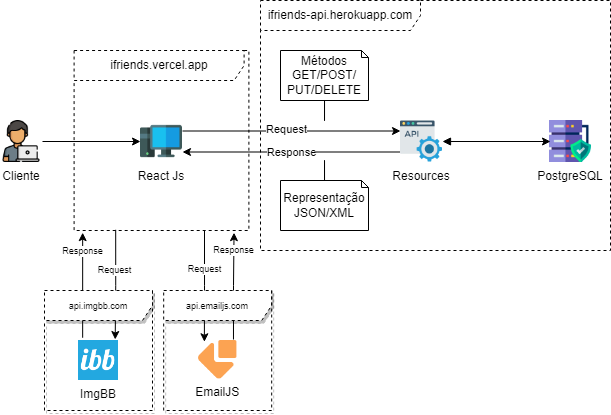
\includegraphics[width=1.0\textwidth]{anexos/Imagens_Diagramas/Arquitetura-Rest-API.png}
\fonte{Os autores.}
\end{figure}
\FloatBarrier

Quanto ao banco de dados, foi utilizado o \gls{postegreSQL}: um \acs{sgbd} popular de \acs{sql}, que serve para executar comandos no banco, como consultas, e alterações nos dados ou na estrutura.

Para hospedar a aplicação, a equipe utiliza o \gls{heroku} para hospedagem da \acs{api} e o \gls{vercel} para a interface de usuário, sendo ambos plataformas em nuvem que suportam diversas linguagens de programação e permitem a implantação, escalonamento e gerenciamento do sistema.

%-------------------------------------------------------------
\section{Ferramentas de apoio}
%-------------------------------------------------------------
Nesta seção serão especificadas as ferramentas a serem utilizadas para a estruturação e organização do sistema Web.

\begin{itemize}
\item \textbf{Notion}: Foi escolhido como plataforma de organização de projetos, pois este possui métodos de gerenciamento de equipe, fornecendo uma interface para vários desenvolvedores trabalharem utilizando o quadro de kanban, assim como o compartilhamento de arquivos, vídeos e artigos; permitindo também notificações via e-mail sobre atualizações do projeto e de reuniões marcadas, por exemplo. 
    
\item \textbf{Discord}: Plataforma de comunicação online escolhida, por ser a mais utilizada e conhecida pelos membros da equipe. Nela é possível criar servidores privados para compartilhar informações e realizar reuniões sobre o projeto.
    
\item \textbf{Overleaf}: Para a preparação do documento de visão, será usado o \LaTeX, visto que este possui comando de padronização para documentos acadêmicos, facilitando a sua construção, juntamente, com editor Overleaf que oferece um ambiente compartilhado entre os membros da equipe. 
    
\item \textbf{Figma}: Na parte de modelagem do sistema e elaboração ideias de soluções de problemas, escolheu-se o Figma, visto que é uma ferramenta gratuita que possui diversas opções de edição.
    
\item \textbf{Visual Studio Code}: A \acs{ide} escolhida para realizar a edição de código-fonte na parte \textsl{\gls{front-end}} do sistema, por razões de ser um recurso da atualidade com possibilidades de várias adaptações de ambiente, principalmente as nossas tecnologias escolhidas.

\item \textbf{Eclipse}: A \acs{ide} escolhida para realizar a edição de código-fonte na parte \textsl{\gls{back-end}}, por motivo de facilidade que o ambiente de desenvolvimento proporciona para rodar aplicações com Java e, também, seus recursos que fazem a integração com o banco de dados.
\end{itemize}

%-------------------------------------------------------------
% -----------------------------------------------------------
\section{Métodos de gestão e desenvolvimento}
\label{metodologia agil}
% -----------------------------------------------------------
Tendo em vista a organização do projeto \gls{ifriends}, a equipe escolheu utilizar os princípios e valores do Manifesto Ágil como norteadores nos seus processos de planejamento, modelagem e desenvolvimento do projeto. Deste modo, elencou-se  o \gls{framework} Scrum como metodologia ágil como referência para o trabalho da Bunka Bytes.

%------------------------------------------------------------
\subsection{Metodologia ágil}
%------------------------------------------------------------
Segundo \citeonline{ambler2004modelagem}, o termo “metodologias ágeis” surgiu em fevereiro de 2001, quando  especialistas em processos de engenharia de \textsl{software} se reuniram e estabeleceram princípios comuns entre todas as metodologias, criando a Aliança Ágil e o estabelecimento do ``Manifesto Ágil'' \textsl{(Agile Manifesto)}.

O termo metodologia ágil consiste na otimização do tempo para a realização de determinado projeto, visando a rapidez na entrega e na qualidade, surgindo assim, como uma resposta mais leve, mais assertiva e menos custosa em relação aos métodos pesados que eram utilizados para a construção de sistemas. Nas metodologias ágeis, os processos, as ferramentas, as documentações, as negociações e os planejamentos, possuem prioridade secundária, pois os indivíduos e suas interações são considerados essências e indispensáveis \cite{sganderla2016aprimorando}.

Para isso, o manifesto determina quatro valores principais, sendo eles: o enfoque nos indivíduos e nas interações, e não nos processos ou algoritmos; a adaptação e maior flexibilidade a novos fatores decorrentes do desenvolvimento do projeto; o foco na funcionalidade do sistema e na documentação mais simples e objetiva, e por último, a preferência por um ambiente de trabalho mais colaborativo e menos burocrático  \cite{sganderla2016aprimorando}. 

Segundo \citeonline{cruz:2018}, o Scrum pode ser definido como ``um \textsl{\gls{framework}} para desenvolver e manter produtos complexos que também pode ser utilizado no gerenciamento ágil de projetos que se destinam também à criação de produtos''. Neste caso, sabida a escolha da utilização de uma metodologia ágil para o gerenciamento do presente projeto, foi decidido aplicá-la com base no Scrum e suas especificações, porém, como a finalidade do trabalho é acadêmica, resolveu-se adaptar algumas de suas características para que a metodologia pudesse ser implementada como uma referência na organização e gestão do projeto. Estas serão explicitadas mais a frente, conforme apresentadas as particularidades do \textsl{\gls{framework}}.

% Dentre as principais características do Scrum, está a divisão do desenvolvimento em ciclos repetitivos e curtos, permitindo modificações, adaptações e correções no produto de forma iterativa e incremental, o que, segundo \citeonline{cruz:2018} permite encontrar desvios mais rápido e com menos impacto. \citeonline{cruz:2018} explica que para que os processos sejam otimizados de tal forma, o Scrum possui ainda três pilares de sustentação: transparência, a inspeção e a adaptação.

Além dos pilares da metodologia, há cinco valores importantes para sua construção e prática durante um projeto: coragem, foco, comprometimento, respeito e abertura.  De acordo com \citeonline{cruz:2018} os valores do Scrum são responsáveis por reforçar os princípios do manifesto ágil, principalmente considerando o comportamento e as pessoas maiores do que os processos e ferramentas. 

%------------------------------------------------------------
\subsubsection{O quadro de kanban}
% -----------------------------------------------------------
% Segundo \citeonline{peinado2007compreendendo}, o nome kanban vem do japonês ``cartão'' e a sua origem deu-se pela seguinte razão:

% \begin{citacao}
% Este nome surgiu em razão do sistema de controle visual dos estoques de materiais, pois são frequentemente utilizados cartões para representar os contentores cheios ou vazios, estes cartões são retirados ou colocados em um quadro à medida que o material é utilizado, ou reposto
% \cite{peinado2007compreendendo}.
% \end{citacao}

% E através da implantação realizada por \citeonline{silva2012beneficios}, devido aos problemas e necessidades encontrados ao longo dos \textsl{Sprints}, houve a criação de um processo ágil, baseado nas práticas do Scrum com características do kanban:

% \begin{citacao}
% As tarefas ou itens de trabalho foram representadas através de cartões (do inglês \textsl{post-its}) fixados em um quadro (do inglês \textsl{cardwall}). 
% Esse quadro, por sua vez, era dividido em colunas que representavam as fases do fluxo de trabalho (do inglês \textsl{workflow}) da equipe. 
% As tarefas eram distribuídas sequencialmente nas colunas à medida que avançavam no fluxo de trabalho \cite{silva2012beneficios}.
% \end{citacao}

No projeto a implementação do kanban foi similar, porém todo o esquema presencial foi adaptado ao quadro remoto. Para conciliar a participação contínua da equipe, a ferramenta \textsl{Notion} é utilizada como auxiliar aos processos de organização, onde também foi possível criar os quadros de kanban do projeto. 

O quadro de kanban usado pela equipe Bunka Bytes foi dividido em dois: no primeiro, encontram-se tarefas (``cartões virtuais'') relacionadas a pendências administrativas e de documentações/mídias, apresentando 5 colunas, nas quais são representadas visualmente em qual estágio a tarefa se encontra, as colunas se classificam como ``para fazer'', ``planejamento'', ``em andamento'', ``para revisar'' e ``feito''.

Já o segundo, possui uma visão global de todas as histórias de usuário que estão sendo trabalhadas na \textsl{Sprint} atual, conforme explicado na \autoref{artefatos}, portando possui raias que variam de acordo com os estados de cada história, sendo eles divididos em: ``para fazer'', ``em andamento'', ``em revisão'', ``pronta'' e ``entregue''. Tal distinção precisou ser feita devido a uma avaliação da equipe sobre demonstrar com maior clareza os itens de \textsl{Backlog} no quadro com os atributos necessários para uma história de usuário enquanto funcionalidades do sistema (como sua pontuação, tamanho, prioridade, critérios de aceitação, descrição e aquém está atribuída), tendo em vista que estes podem ser diferentes daqueles utilizados em tarefas mais administrativas.

Desse modo, para ambos a priorização é um item em comum e deve seguir um padrão, por isso foi decidido utilizar uma classificação em ordem de prioridade para cada tarefa/história, podendo ser ``alta'', representada pela cor vermelha, ``média'', representada pela cor laranja, e ``baixa'' representada pela cor verde, tais prioridades são atribuídas às tarefas/histórias assim que a entrega é planejada.

De maneira geral, o uso do quadro de kanban é beneficial ao projeto, já que através de sua aplicação a equipe consegue conciliar de maneira clara e precisa as tarefas/histórias compartilhadas. A utilização do quadro remotamente e através do Notion, faz com que a equipe possa ainda acessá-lo de qualquer lugar, facilitando o processo de transparência dos itens e faz com que todos tenham em usas mão as atividades a serem feitas, podendo ajustá-las quando preferirem. 

%------------------------------------------------------------
\section{Gestão da equipe}
% -----------------------------------------------------------
A equipe Scrum é composta por três papéis: o \textsl{Scrum Master}, o \textsl{Product Owner} e o Time de Desenvolvimento:

\begin{citacao}
O primeiro, chamado \textsl{Scrum Master}, é considerado o responsável por garantir que o Scrum seja entendido e aplicado, para que o Time Scrum esteja aderindo os valores, as práticas e as regras do Scrum, e, portanto, trabalha como um líder ou técnico da equipe. Já o \textsl{Product Owner}, é o principal responsável pelo gerenciamento do \textsl{backlog} do produto, por garantir o valor do trabalho realizado pelo Time, e pela satisfação e atendimento das necessidades do cliente. O Time de Desenvolvimento, por outro lado, é responsável por executar o desenvolvimento e transformar o \textsl{backlog} do produto em incrementos de funcionalidades, criando um sistema pronto que possa ser entregue ao cliente \cite{cruz:2018}.
\end{citacao}

Portanto, para fins de organização, o Time de Desenvolvimento deve ser dividido em subequipes, sendo elas: desenvolvimento, design e documentação, e mídias. Nelas, estão inclusas as funções de desenvolvedores \gls{front-end} e \gls{back-end}, divididas entre os integrantes Jamilli Vitória Gioielli, José Roberto Claudinho Ferreira e Kaiky Matsumoto Silva; sendo a Jamilli e o José responsáveis por supervisionar o \gls{front-end} da aplicação, e o Kaiky pela supervisão do \gls{back-end} - que também inclui a administração do banco de dados. Porém, os três atuam de formas diretas ou indiretas em ambas as partes do desenvolvimento.

Além dessas, as outras duas subequipes foram dividias entre as integrantes Anaí Villca Rojas, responsável  por supervisionar o design de experiência/interface de usuário; e Julia Romualdo Pereira, responsável pelo gerenciamento da documentação e das mídias do projeto (como o canal no \gls{youtube} e as postagens no Blog). 

De todo modo, a documentação e as mídias do projeto deverão ser revisadas, obrigatoriamente por todo o time, de modo a manter um conhecimento sobre a aplicação melhormente distribuída. Entretanto, precisa-se compreender que a modelagem de dados e a elicitação de requisitos da aplicação foram feitas com o auxílio de todos os integrantes, visto que são partes de extrema importância para que a compreensão de todos sobre o cenário corresponda com o objetivo principal pretendido. No \autoref{distribuicao_tarefas}, é possível observar uma relação das supervisões dos integrantes em cada área do projeto. 

\begin{quadro}[htb]
\centering
\ABNTEXfontereduzida
\caption{Distribuição de tarefas}
\label{distribuicao_tarefas}
\resizebox{\linewidth}{!}{

\begin{tabular}{|l|c|c|c|c|}
\hline

\thead{Responsável} & \thead{Front-end} & 
\thead{Back-end}  & \thead{Documentação e Mídias} & \thead{Design}\\
\hline
Anaí &    &    & \circlemark & \circlemark \\
\hline
Jamilli & \circlemark &  &  & \circlemark \\
\hline
José & \circlemark &  &  &   \\
\hline
Julia &  &  &  \circlemark &  \\
\hline
Kaiky & & \circlemark &  &  \\
\hline

\end{tabular}}\legend {Fonte: Os autores.}
\end{quadro}
\FloatBarrier 

Entretanto, é importante salientar que as funções atribuídas a cada um não são exclusivas e podem variar conforme a necessidade de entrega do projeto. As subequipes são de responsabilidade de todos os integrantes e apenas foram divididas assim para fins de organização das tarefas do projeto. Levando isso em consideração, as funções de \textsl{Scrum Master ou Iteration Manager} e \textsl{Product Owner} foram adaptadas, ainda que não seja o ideal na metodologia ágil, para um único papel, representado pela integrante Jamilli Vitória Gioielli. Porém, vale ressaltar ainda que, nesse modelo escolhido, toda a equipe é responsável pela inspeção dos processos do projeto, e não somente o \textsl{Scrum Master ou Iteration Manager}:

\begin{citacao}
O Time deve ser multidisciplinar e multifuncional, possuindo todo o conhecimento necessário para criar um incremento no trabalho. [...] Não há títulos no Time, e não há exceção a esta regra. Não deve existir distinção de cargos ou funções, títulos ou senioridades, e muito menos áreas determinadas ou específicas de atuação. No Scrum todos os integrantes do Time são conhecidos como “desenvolvedores”.

Individualmente, os integrantes do Time de Desenvolvimento podem ter habilidades específicas, mas, independentemente disso, a responsabilidade a respeito de uma entrega continua sendo do Time de Desenvolvimento como um todo \cite{cruz:2018}.
\end{citacao}

Para organizar a produtividade contínua de desenvolvimento do projeto, buscando seguir uma das vertentes propostas na metodologia ágil de entregas semanais, a equipe criou um cronograma de entregas por aula baseado a partir do plano de ensino da disciplina disponibilizado pelos orientadores, ou seja, a equipe busca realizar durante a semana a atividade proposta para a aula seguinte para aproveitar o tempo em sala de aula validando o que foi realizado com os orientadores. 

O cronograma de entrega semanal utilizado para o desenvolvimento do projeto \gls{ifriends} pode ser observado na \autoref{cronograma_desenvolvimento}.

\begin{figure}[htb]
\centering
\caption{Cronograma de Desenvolvimento Semanal}
\label{cronograma_desenvolvimento}
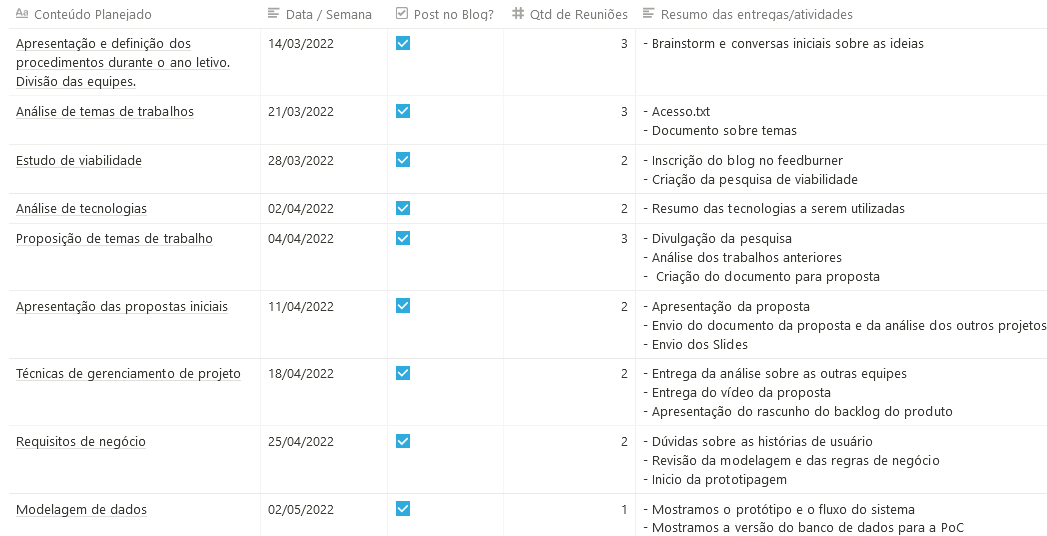
\includegraphics[width=1.0\textwidth]{anexos/Imagens_Proposta/cronograma_desenvolvimento.png}
\fonte{Os autores.}
\end{figure}
\FloatBarrier

%------------------------------------------------------------
\subsection{Artefatos e eventos utilizados}
\label{artefatos}
%------------------------------------------------------------
Tendo em vista a finalidade acadêmica do projeto, foi estipulado um valor mínimo de duas reuniões semanais dedicadas na construção, considerando a organização individual de cada membro da equipe, além da priorização para que a tomada de decisões e planejamentos sejam feitas no dia das aulas da disciplina de \acs{pds}. Sobre os artefatos e eventos do Scrum, lista-se a seguir suas funcionalidades originais, descritos por \citeonline{cruz:2018}, e como serão adaptados:

\begin{itemize}
\item \textsl{Backlog}: é descrito como uma lista de todas as características, funções, tecnologias, melhorias e correções que constituem o produto a ser entregue. É também subdividido em ``do produto'', ``da versão de entrega'' e ``da \textsl{Sprint}'';

\item \textsl{Sprint}: originalmente pensada para durar um mês ou menos e possuir uma meta estabelecida com um objetivo claro, foi pensada 
para durar até duas semanas, já que as orientações da disciplina exigem que existam entregas frequentes, isto é, todas as semanas. Portanto, o ideal é que se dê início ao trabalho a ser entregue pelo menos uma semana antes de sua entrega;

\item \textsl{Time-boxed}: é esperado que o tempo estipulado para executar uma tarefa seja cumprido e que o trabalho proposto, seja realizado. Tendo em vista os curtos prazos,
também foi adaptado conforme a entrega;

\item Planejamento da \textsl{Sprint}: ainda será utilizado para definir ``o que será feito'' e ``como'', porém, ao contrário das oito horas mínimas 
estipuladas, a equipe definiu um mínimo de duas horas para tal reunião, que poderá acontecer nas segundas-feiras, durante a aula de \acs{pds} ou aos finais de semana, logo após a finalização dos entregáveis;

\item Reuniões Diárias: não serão mantidas de maneira síncrona, visto que cada membro da equipe possui horários de disponibilidade diferentes. Porém, poderão ocorrer de forma assíncrona, de modo a compreender se existem impedimentos durante a execução das tarefas planejadas para a semana;

\item Revisão da \textsl{Sprint}: seu maior objetivo é a revisão do \textsl{Product Owner}, ou do cliente, em todos os itens concluídos pelo Time. Porém, 
não terá \textsl{Time-boxed} de quatro horas, visto que a aprovação dos professores orientadores (o cliente) pode ser mais rápida e acontecer durante a execução das tarefas. No entanto, a equipe a realizará em todo final de entrega, para que os retornos dos professores levem em consideração o trabalho final;

\item Retrospectiva da \textsl{Sprint}: possui originalmente \textsl{Time-boxed} de até três horas e é feita para identificação 
de medidas de melhoria no processo do time que serão aplicadas na próxima \textsl{Sprint}. Foi escolhido adaptá-la para acontecer às terças-feiras, antes do início das aulas, para que as entregas feitas às segundas-feiras estejam frescas e o processo realizado pelo time possa ser mais bem avaliado para a melhoria contínua.
\end{itemize}

Para a definição do \textsl{backlog} do produto, o Scrum conta com um recurso chamado histórias de usuário, que pode ser definido como: 

\begin{citacao}
História é uma descrição resumida, porém clara e objetiva, de alguma funcionalidade que deverá ser fornecida pelo produto a ser entregue, sempre do ponto de vista do usuário final. Uma história não é uma especificação completa da funcionalidade, mas uma promessa de discutir uma funcionalidade, ou, simplesmente, um lembrete de que a discussão já aconteceu. Um modelo simples de como escrever uma história seria: ``Como um <tipo de usuário>, eu quero <um objetivo> para que <atenda a uma necessidade>'' \cite{cruz:2018}.
\end{citacao}

% Entretanto, vale ressaltar que as histórias de usuário do presente projeto serão montadas somente na parte de desenvolvimento, isto é, quando o produto começar a ser construído pelo Time Scrum e após os principais itens de \textsl{backlog} estarem descritos. Como ainda se encontra na fase de planejamento e modelagem, tal recurso ainda não foi acionado no projeto.

Entretanto, vale ressaltar a respeito a utilização do \textsl{Scrum Poker} ou \textsl{Planning Poker Card}, que, segundo \citeonline{cruz:2018}, é definido como ``uma técnica que auxilia na estimativa de histórias e tarefas com base no consenso de todo o Time''. Para tanto, o Time utiliza um conjunto de cartas com valores representando os pontos ou horas por história. Sobre o funcionamento do \textsl{Planning Poker Card}:

\begin{citacao}
O seu uso é simples: o \textsl{Product Owner} ou um membro do Time apresenta a história, ou tarefa. Após uma breve discussão, cada um escolhe uma carta e a coloca virada sobre uma mesa, de forma que um não constate o valor da carta que o outro escolheu. Quando todos colocarem suas cartas, elas são desviradas para que todos vejam os valores.

Caso não haja consenso entre as cartas escolhidas, as diferenças são discutidas brevemente e uma nova rodada acontece, até que haja convergência e consenso \cite{cruz:2018}.
\end{citacao}

Para o presente projeto, o \textsl{Planning Poker Card} foi utilizado durante o processo de desenvolvimento do produto e após as histórias de usuário da \textsl{Sprint} estarem bem descritas. Vale ressaltar que este processo é apenas para estimar o trabalho da equipe e pode variar conforme o andamento do projeto.

%------------------------------------------------------------
\subsection{Métricas de Desenvolvimento}
%------------------------------------------------------------
De modo a fazer nosso processo de desenvolvimento o mais produtivo possível, e entregar o máximo do \textit{backlog} do produto, foram definidas as seguintes pontuações (\autoref{Métricas}) para identificar o grau de complexidade das tarefas de modo a priorizar o desenvolvimento daquelas que exijam um trabalho maior. Essas pontuações foram baseadas no princípio do \textit{Planning Poker Card}, no qual a pontuação das cartas usadas para a estimativa segue a sequência de \textit{Fibonacci}. 

\def\arraystretch{2}
\begin{quadro}[htb]
\centering
\ABNTEXfontereduzida
\caption{Métricas de Organização das Histórias}
\label{Métricas}
\resizebox{\linewidth}{!}{
\begin{tabular}{|c|c|p{10cm}|}
\hline
\thead{Pontuação} & \thead{Tamanho} & \thead{Descrição} \\ \hline

< 5  & Pequeno & Pontuação usada para classificar tarefas que são de nível fácil e que podem ser realizadas em um curto período. \\ \hline
5 e 8 & Médio & Pontuação usada para classificar tarefas de nível médio e exigem um desempenho maior comparada com as de nível fácil, mas não chegam a ser muito complexas. \\ \hline
$ \geq 13 $ & Grande & Pontuação usada para classificar tarefas que são de nível difícil e exigem um grande desempenho, além de precisarem de mais tempo para serem desenvolvidas. \\ \hline

\end{tabular}}\legend{Fonte: Os autores}
\end{quadro}
\FloatBarrier

Esses critérios de pontuação foram aplicados as histórias de usuário (\autoref{historias de usuario}), portanto, com o uso dessas métricas é possível priorizar tarefas mais complexas (com maior pontuação) das mais simples (com menor pontuação) além de ajudar na execução das \textsl{Sprints}. A aplicação dessas métricas pode ser constada na figura \autoref{metricas_historias}.

\begin{figure}[htb]
\centering
\caption{Histórias no Notion}
\label{metricas_historias}
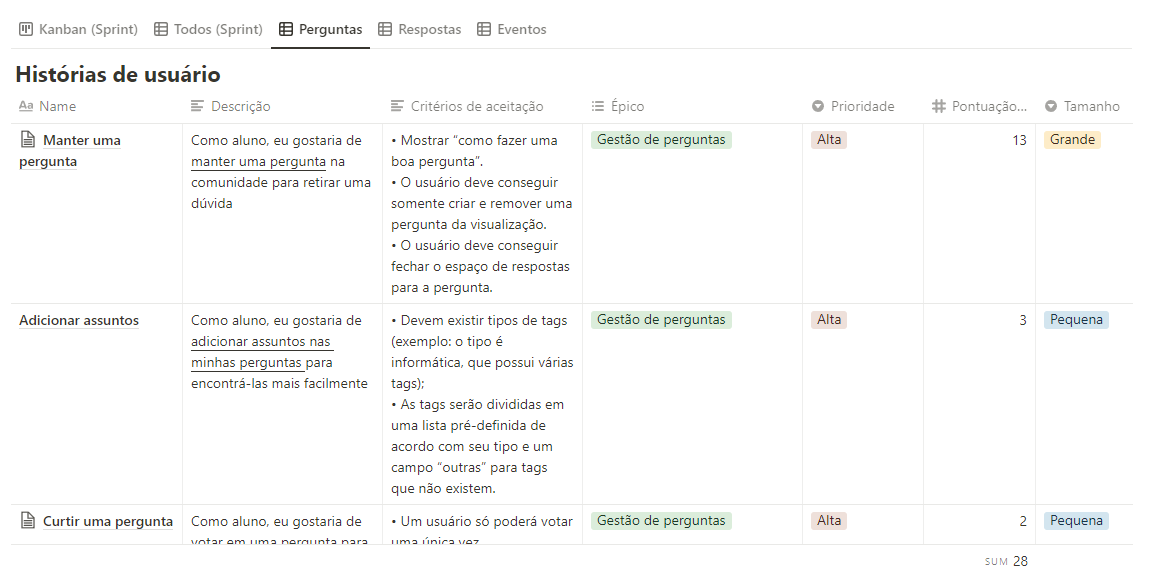
\includegraphics[width=1.0\textwidth]{anexos/Imagens_Desenvolvimento/metricas_historias.png}
\fonte{Os autores.}
\end{figure}
\FloatBarrier

A sua utilização se deu através de uma reunião realizada por todos os membros da equipe e como o auxílio do \href{https://www.scrumpoker-online.org/en/}{Scrum Poker Online} que nos forneceu as ferramentas necessárias para realizar a estimativa de pontuação.

%------------------------------------------------------------

%-------------------------------------------------------------